\section{Workflow pipelines}\label{sec:workflow}

\subsection{DevOps CI/CD pipelines}\label{subsec:ci/cd-pipelines-and-development-workflow}
As we explained while describing the infrastructure, part of our global workflow can be implemented within pipelines runners definition.
We used GitHub action and the GitHub flow to harmonise the workflow within our different type of git repositories.
GitHub allows us to define template in a single repository that can be then versioned and used in other repositories while hiding the complexity of the defined pipelines.
We also followed the GitHub flow which involve one main branch and features or hotfix branch to favor small and fast releases.
As stated before other strategies can be used with an adapted development workflow.

\begin{figure}[!htbp]
    \centering
    \caption{Implementation of the GitHub Flow CI/CD workflow}
    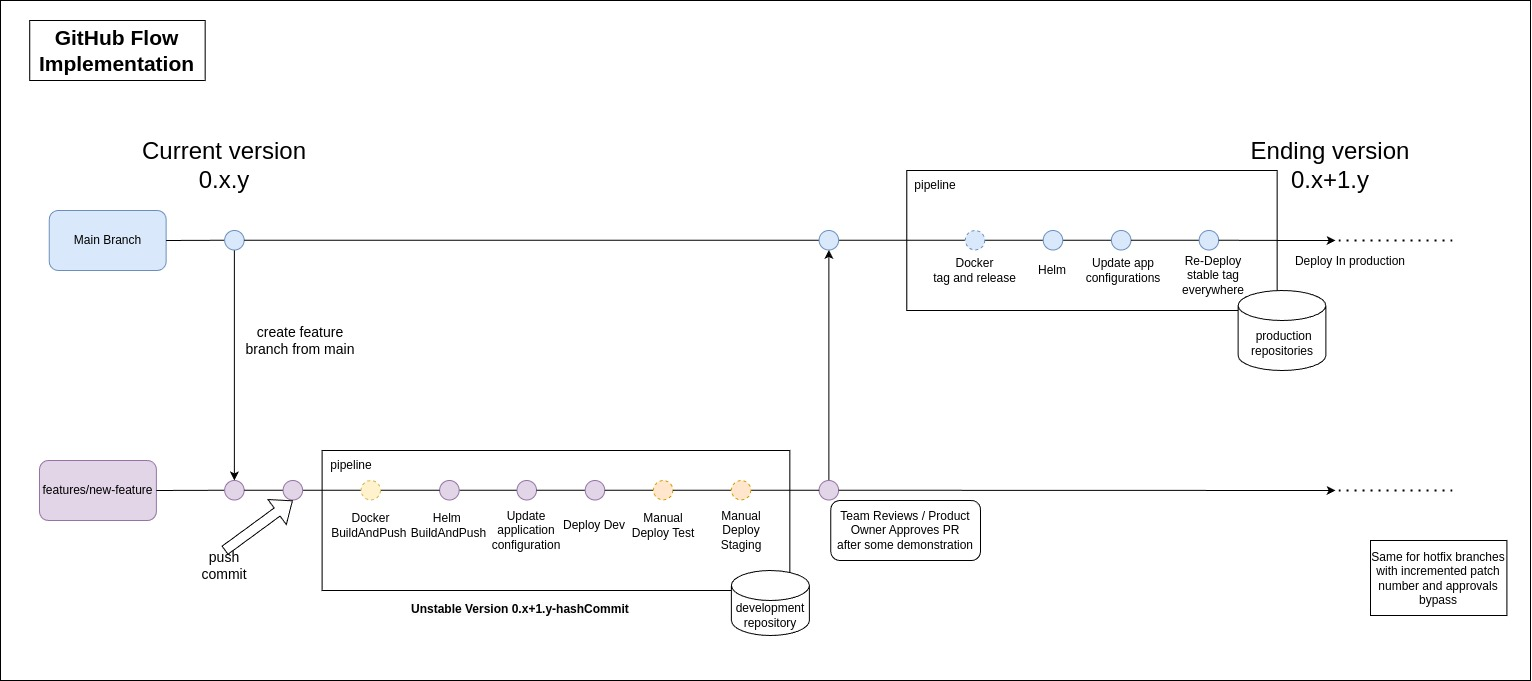
\includegraphics[scale=0.3]{images/project/cicd-workflow-p1}
    \label{fig:cicd-workflow-p1}
\end{figure}

Our DevOps workflow, following the GitHub flow, requires that new development be done on a separate branch.
The project version is incremented, and the commit hash is appended to the version string.
Unit tests are performed during the build phase within the Docker image to ensure code quality.
This versioned build can then be deployed to each environment, where further tests are executed using ArgoCD and Helm test definitions.
Once a merge request is accepted, the commit hash is removed from the version, and the images are either rebuilt or retagged with the new version.
Additionally, the repository is tagged to facilitate rollback if necessary.
Creating a pull request allows developers to facilitate collaboration and verification before deploying to production.
(See Figures \ref{fig:cicd-workflow-p1} and \ref{fig:cicd-workflow-p2})

\begin{figure}[!htbp]
    \centering
    \caption{Development Team Contribution activity}
    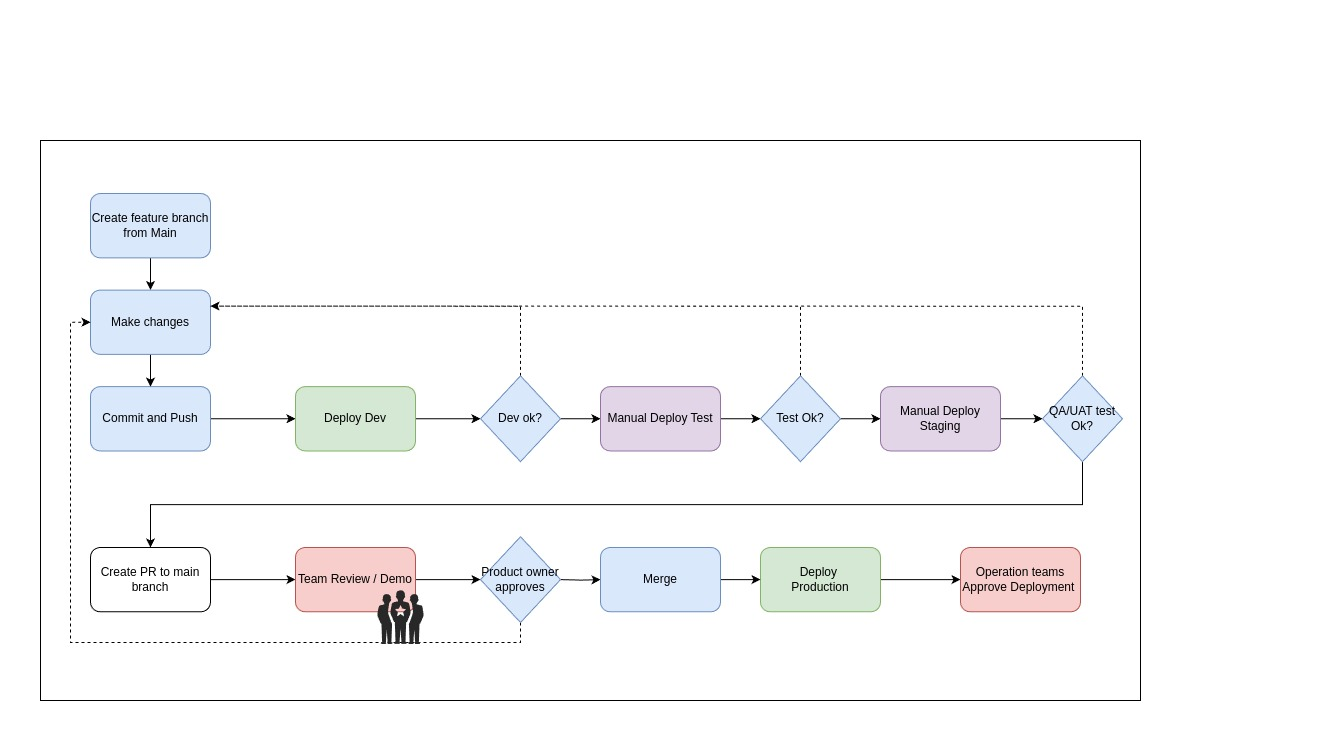
\includegraphics[scale=0.3]{images/project/cicd-workflow-p2}
    \label{fig:cd-workflow-p2}
\end{figure}

There are our development pipelines for any git repositories except for the deployment repository that are only targets.
Artifact that are not deployed but released to a repository follows the same path but are deployed as dependencies within other projects.
Airflow DAGS and Kubeflow pipelines follows the same development workflow and are release into our previously defined git deployment repositories.

% image of github action runners.

\subsection{DataOps pipelines}\label{subsec:dataops-pipelines}
Inspired by our research in the literature we create a sample DataOps pipeline that can be implemented with specific
operations.

\begin{figure}[!htbp]
    \centering
    \caption{DataOps sample workflow}
    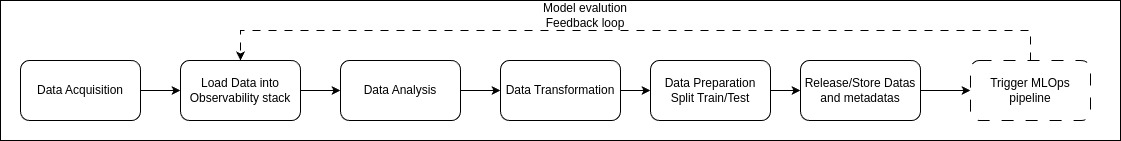
\includegraphics[scale=0.3]{images/project/dataops-workflow}
    \label{fig:project-dataops-workflow}
\end{figure}

It's defined in our project as an Airflow DAG and can be triggered manually in early stage of the project or
automatically when the project has enough maturity.

Each step of the pipeline can be defined as a container image using the Airflow Domain specific language (e.g.\ ContainerSpec).
We use the same parameter definition strategy outlined in our model development section (\ref{subsec:model-development}),
so that each step in the pipeline can be easily replaced with an alternative implementation.

\begin{figure}[!htbp]
    \centering
    \caption{DataOps workflow define in Airflow}
    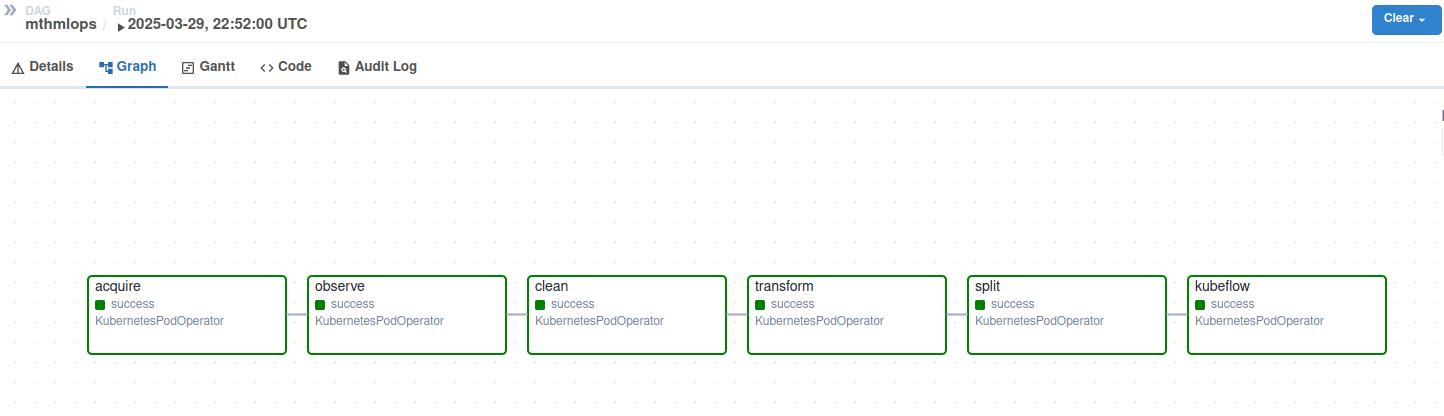
\includegraphics[scale=0.3]{images/project/dataops-workflow-airflow}
    \label{fig:dataops-workflow-airflow}
\end{figure}

Also, by defining all our steps as independent containers, we decouple them from the pipeline orchestrator.
This flexibility allows us to implement steps in different languages if better suited for our Data or Machine Learning teams.

One disadvantage is the additional time required to start a new container for each step.
However, this overhead is often negligible, as Data and Machine Learning steps typically take a long time to run.

We demonstrate this flexibility by replacing our original data-collector dummy step with the LSFB dataset library\cite{9534336}, encapsulated within a container.
Since the LSFB dataset comes pre-split and prepared, we can skip several steps in our DataOps pipeline.

Below, we provide a detailed explanation of each step in our pipeline.

\subsubsection{Acquire}
Data is collected from external sources or internal repositories.
We use containers with parameters to set appropriate location per project.

\subsubsection{Observe}
Initial analysis is performed to understand the data's structure and content.
In this step we load the data into an observability stack (ElasticSearch or OpenSearch for example)

\subsubsection{Clean}
Missing values are handled and inconsistencies are corrected.

\subsubsection{Transform}
Within this step we format the data according to project requirements.

\subsubsection{Split}
We then divide and release the dataset into training, validation, and test sets.

\subsubsection{MLOps pipeline Triggers}
Airflow triggers the Kubeflow pipeline to initiate the MLOps workflow.

\subsection{MLOps pipelines}\label{subsec:mlops-pipelines}
Our MLOps pipelines are developed as Kubeflow pipelines with the possibility to trigger them from an airflow DAG
even in the early stage of the project.
This ensures the possibility of combining it with the DataOps pipeline, facilitating further automation.

\begin{figure}[!htbp]
    \centering
    \caption{MLOps workflow in Kubeflow pipelines}
    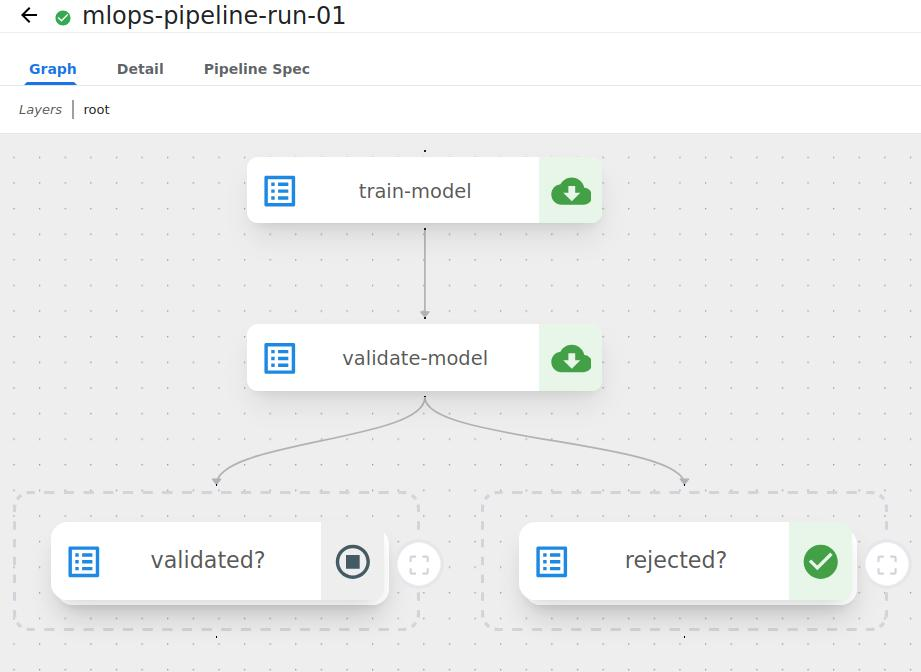
\includegraphics[scale=0.3]{images/project/mlops-workflow-kubeflow}
    \label{fig:mlops-workflow-kubeflow}
\end{figure}

In our MLOps workflow, we have established a seamless integration between Apache Airflow and Kubeflow Pipelines to
efficiently manage the machine learning lifecycle.
This integration automates the process from data availability to model deployment, ensuring a streamlined and reproducible workflow.

Each step of the pipeline is defined as a container image using the Kubeflow Pipelines domain-specific language (e.g., ContainerSpec).
We follow the same design principles as in our DataOps pipeline,
enabling easy replacement of individual steps and flexibility to use different languages when appropriate.
This container-based modularity also ensures less coupling with the pipeline orchestrator.

\subsubsection{Model Training}
The pipeline begins with a training component that uses the datasets provided by our DataOps pipeline to train a machine learning model.

\subsubsection{Model Validation}
After training, a validation component assesses the model's performance using the test data.
If the model meets our predefined accuracy thresholds and/or performs better than previous models,
the workflow proceeds; otherwise, it terminates, ensuring only validated models advance to production.

\subsubsection{Release model}
Upon successful validation, the pipeline enters the release phase, where the model and its metadata are saved to MinIO\@.
The deployment component updates our production environment with the new model, ensuring minimal disruption and continuous service delivery.
The model is released along with its metadata, which currently includes primarily accuracy and versioning information.

\subsubsection{Reject the model}
If validation fails, the pipeline is halted, and no updates are made to the model or its metadata.
The production environment remains intact, preventing any disruptions and maintaining continuous service.

\subsubsection{Deploy}
This part is crucial in our implementation as instead of using Kubeflow serve capabilities we rather use a GitOps methodology
and use this step to commit configuration changes in our configuration git repository that is synced by ArgoCD
using the deployment strategy define in the deployment or rollout manifest within our HelmChart.
In addition, with our helm tests we can run our integration tests before,
during or after the deployment to ensure a successful deployment in any environments.
This way we ensure consistency between all our deployments. % and we are happy :)
ArgoCD notifications can close the loop by confirming the deployment through a webhook call.
